
\section{Handshake circuits}


One of the approaches to design of asynchronous circuits is syntax-directed mapping with 
handshake circuits as an intermediate format. The parse tree of a program source code written in 
a CSP-style \cite{csp} language can be interpreted as a graph of components, connected with communication links
called handshake channels. The components can then be individually mapped to gate-level implementations
with complete circuit derived by implementing the handshake channels with wires.

This approach has been first used by Philips in their Tangram \cite{tangram} design tool
and later made publicly available after the similar free Balsa \cite{balsa} system has been released.

This thesis will be working with Balsa handshake components.

A handshake activation $h$ is said to \emph{enclose} a process $p$ if $p$ can only start after $h$ gets a request and $h$ can get an acknowledgement only after $p$ gets finished.

A \emph{handshake circuit} consists of handshake components which interact by request/acknowledgement handshaking 
over communication channels.
Each \emph{handshake component} is specified by a set of ports and a process communicating over those ports.
A \emph{protocol} is assigned to each port, which specifies whether the process initiates the handshakes
over an \emph{active port} or awaits for the other party over a \emph{passive port}. 
It also specifies the direction and size of data transferred during the handshakes.
Each \emph{channel} connects two ports of the same data size with one port being active and the other being passive.

On diagrams used in this thesis we display handshake components with large circles with a process symbol inside
and handshake ports with small circles where filled circle stands for active port and hollow circle stands for passive port.
Channels are displayed as lines between the corresponding ports with the direction of the arrow corresponding to the
direction of data flow.


The defining feature of a handshake component is the process associated with it. 
In Balsa there are about fifty types of processes with each 


\begin{itemize}
\item
Sequence is a component with three control ports: a passive port $s$ and two active ports $t_1$ and $t_2$.
The behaviour of the component is as follows: upon receiving an activation it encloses the two activations activation of $t_1$ action   awaits for activation over $s$ and encloses the following: a handshake over $activate_1$ followed by a handshake over $activate_2$; after receiving the acknowledgement  and acknowledges

\item
Concur is a component with a similar external interface: it has a passive port $activate$ and two active ports $activate_1$ and $activate_2$.
The behaviour during the activation on $activate$ is to activate $activate_1$ and $activate_2$ in parallel.
\end{itemize}



\begin{figure}
\centering
\subfloat[Sequence\label{fig:SequenceOptimised}]{
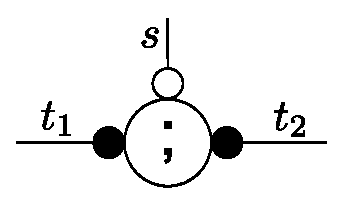
\includegraphics[scale=0.5]{figures/Control/sequence-HC}
} {}
\subfloat[Concur\label{fig:Concur}]{
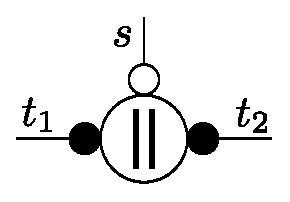
\includegraphics[scale=0.5]{figures/Control/concur-HC}
} {}
\subfloat[BinaryFunc\label{fig:BinaryFunc}]{
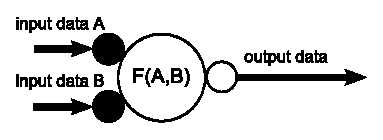
\includegraphics[scale=0.4]{figures/Data/binaryfunc-HC}
} {}
\subfloat[CallMux\label{fig:CallMux}]{
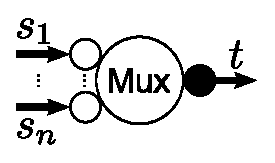
\includegraphics[scale=0.5]{figures/Data/callmux-HC}
} {}
\subfloat[Variable\label{fig:Variable}]{

\includegraphics[scale=0.5]{figures/Data/variable-HC}
} {}
\subfloat[While\label{fig:While}]{
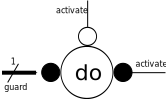
\includegraphics[bb=0bp 0bp 134bp 80bp,scale=0.5]{figures/while-HC}
} {}
\subfloat[Case\label{fig:Case}]{

\includegraphics[scale=0.5]{figures/case-HC}
}

\caption{Handshake components}
\end{figure}





 Each channel connects two ports. Each port is connected to a channel. 
with which it
can be connected point-to-point to a port of another handshake circuit by means of a channel. 
. Each
channel carries request and acknowledgement signalling as well as an optional data payload. The
requests flow from the active component ports (filled circles) towards passive component ports
(open circles). Acknowledgements flow in the opposite direction to requests. Where a channel
carries data, the direction of the data is indicated by an arrow on that channel’s arc. The direction
of data may be different from the direction of signalling to support push and pull port and channels.
A handshake component can be activated by sending request to its passive port. When activated, 
it sends requests to a subset of its active ports and waits for acknowledgements. The
subset of the ports activated by the component is determined by its function and may be data-
dependent. The order in which the component activates its ports is shown by small numbers next
to the ports. The ports of a handshake component which are marked with the same number are ac-
tivated concurrently. When all activated ports are acknowledged, the handshake component sends
an acknowledgement to the passive port from which it was activated and finishes its operation until
the next activation.
